\section{$S=1$ Magnetometry}\label{s1_magnetometry}
We will consider the use of a SiC divacancy e.g. PL5 or PL6.

We begin with our total Hamiltonian \eqref{eq:total_hamiltonian}. We will consider the system under the influence of only the $\vec{B}$ field, so can remove the Stark effect terms. Additionally, for $S=1$ we may reduce the constant terms \cite{Christle2014} leaving
\begin{equation}
	H = g\mu_b \hat{\vec{S}}\cdot\vec{B} + D\hat{S}_z^2 + E (\hat{S}_x^2 - \hat{S}_y^2).
	\label{eq:s1_magnetometry_hamiltonian}
\end{equation}

By transforming into spherical coordinates, with $\theta, \phi$ the azimuthal and polar angle respectively and $B = |\vec{B}|$
\begin{equation}
	\begin{align}
		B_x & = & g\mu_b B \cos\varphi \sin\theta \\
		B_y & = & g\mu_b B \sin\varphi \sin\theta \\
		B_z & = & g\mu_b B \cos\theta
	\end{align}
	\label{eq:polar_transform}
\end{equation}
then substituting the spin operators \eqref{eq:s1_spin_operators} we find
\begin{equation}
	H = \begin{pmatrix}
		D + g\mu_b B \cdot \cos \theta                                       & \frac{g\mu_b B}{\sqrt{2}} \cdot e^{-i\cdot \varphi} \cdot \sin\theta & E                                                              \\
		\frac{g\mu_b B}{\sqrt{2}} \cdot e^{i \cdot \varphi} \cdot \sin\theta & 0                                                                    & \frac{g\mu_b B}{\sqrt{2}} e^{-i\cdot \varphi} \cdot \sin\theta \\
		E                                                                    & \frac{g\mu_b B}{\sqrt{2}} \cdot e^{i \cdot \varphi} \cdot \sin\theta & D - g\mu_b B \cdot \cos \theta
	\end{pmatrix}.
	\label{eq:s1_magnetometry_hamil_spherical_matrix}
\end{equation}



\subsection{$\vec{B}$ Parallel to Defect}
It is straightforward to show from \eqref{eq:s1_magnetometry_hamil_spherical_matrix} that if the magnetic field is applied parallel to the defect axis ($\theta = 0$) then the matrix reduces to
\begin{equation}
	H_{} = \begin{pmatrix}
		D + g\mu_b B & 0 & E          \\
		0            & 0 & 0          \\
		E            & 0 & D-g\mu_b B
	\end{pmatrix},
	\label{eq:reduced_H_s1_magnetometry_matrix}
\end{equation}
with eigenvalues

\begin{equation}
	E_x = E_y = D \pm \sqrt{(g\mu_b B)^2  + E^2}, \; E_z = 0.
	\label{eq:reduced_H_NV_eigenvalues}
\end{equation}

The uniaxial symmetry of the SiC divacancy means $D \ll E$. Further, we expect to sense in the range where $g\mu_b B \gg D$ therefore we may write the eigenvalues as
\begin{equation}
	E_x = E_y \simeq D \pm g\mu_b B, \; E_z = 0.
	\label{eq:reduced_H_NV_eigenvalues}
\end{equation}

{\color{edired}That is, for the transitions between $m_s=0$ and $m_s = \pm 1$\footnote{These are the allowed transitions for optical depopulation due to selection rules. This may be simply thought of as a helicity conservation as the photon is a $S=1$ particle.}, the difference is energy reflected in the EPR spectra (visualised in figure \ref{fig:linear_zeeman}) is the Zeeman energy
\begin{equation}
	\Delta E = g \mu_B B =  \gamma B.
	\tag{\ref{eq:zeeman_energy}}
\end{equation}
}
\begin{figure}[H]
    \begin{center}
        % 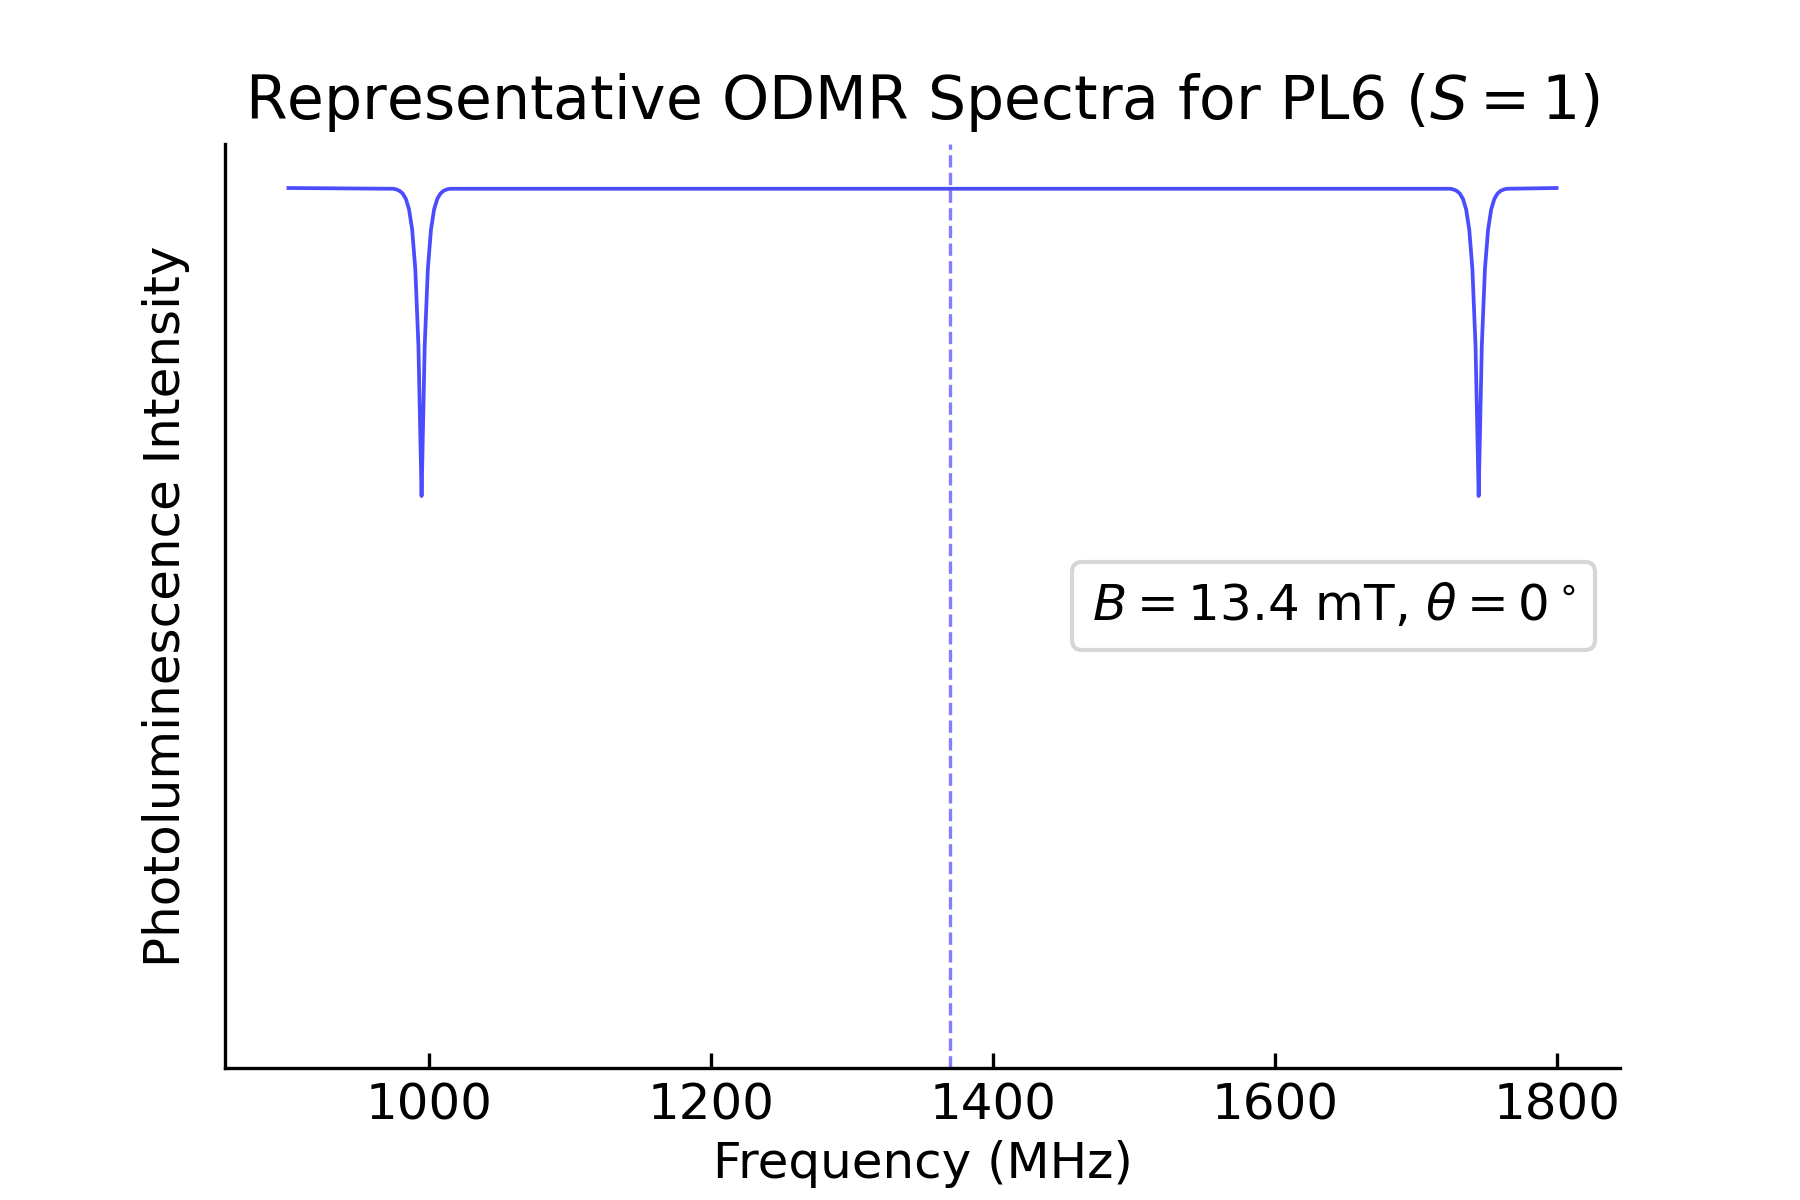
\includegraphics[width=0.49\textwidth]{figures/ODMR-s1magnet-1.png}
        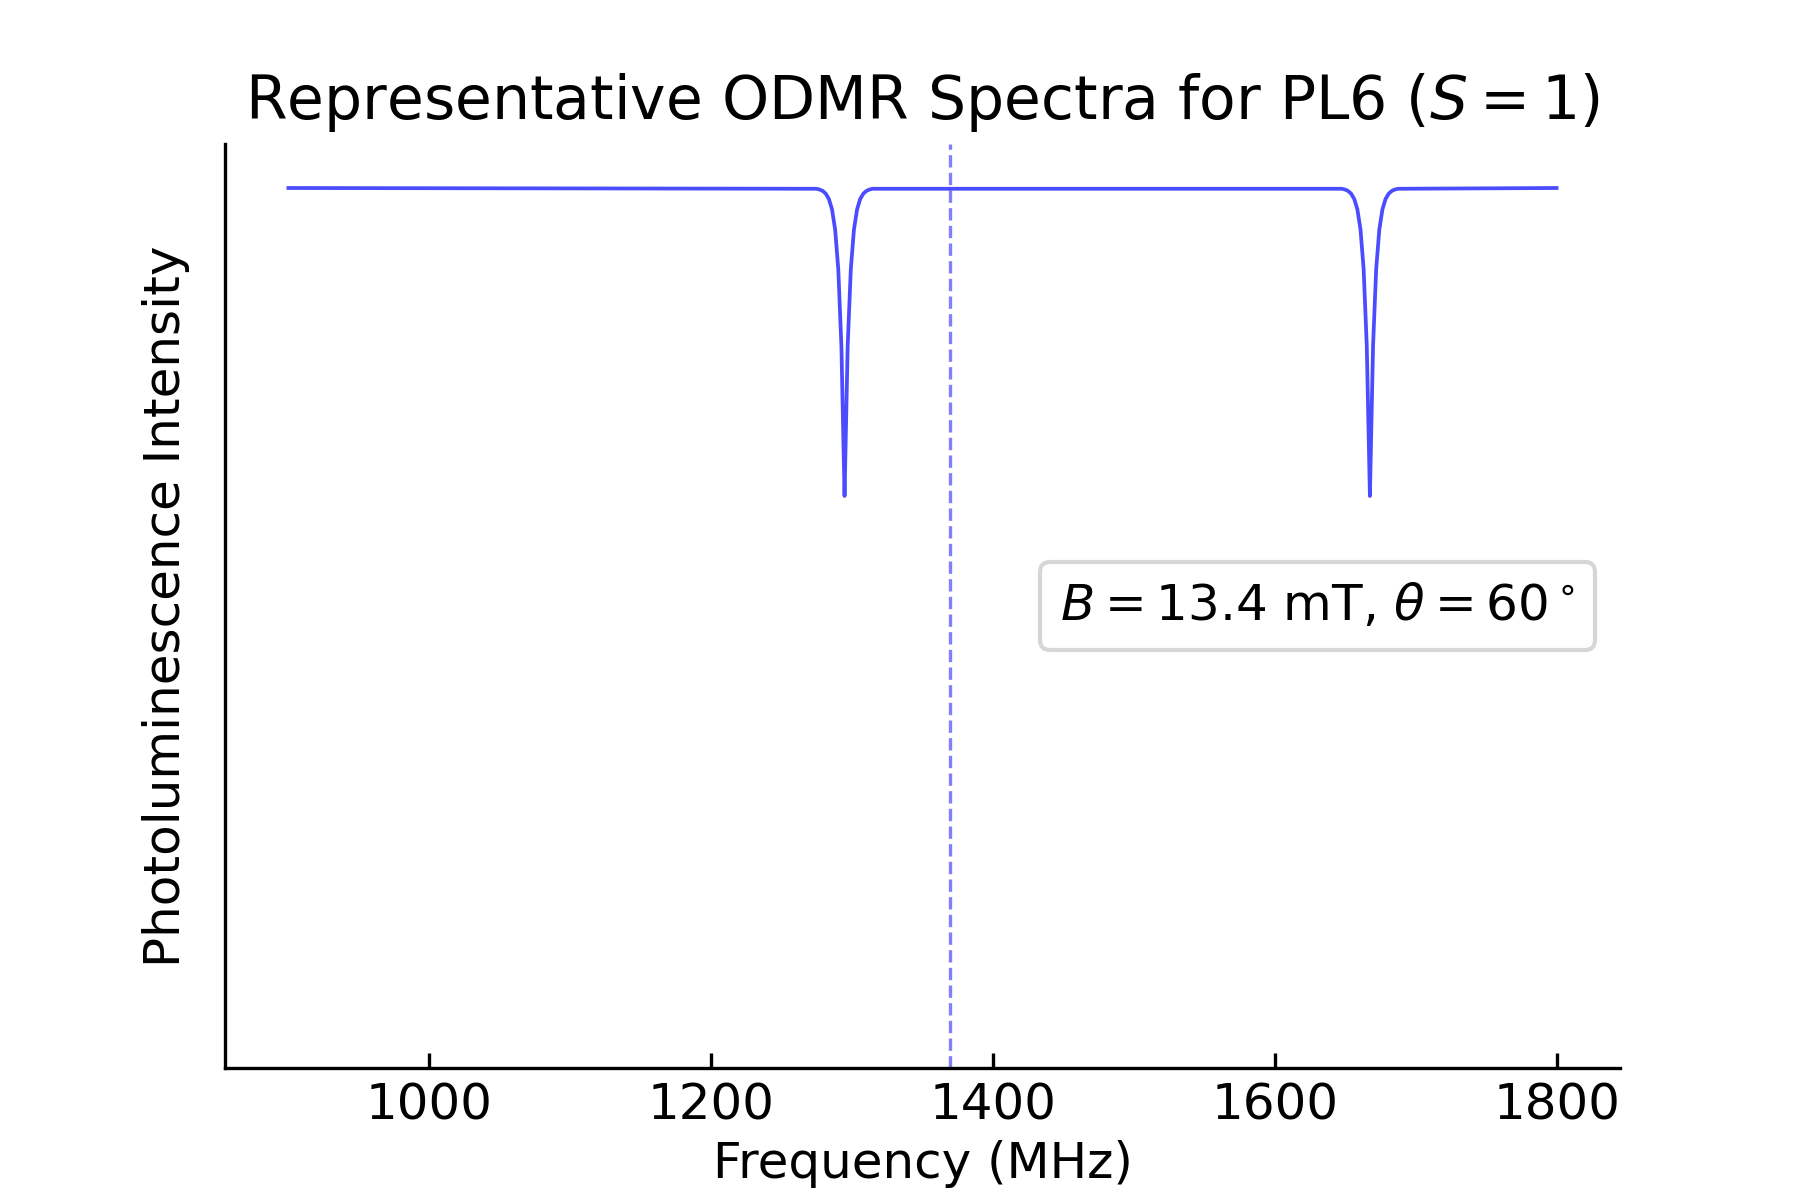
\includegraphics[width=0.49\textwidth]{figures/ODMR-s1magnet-2.png}
        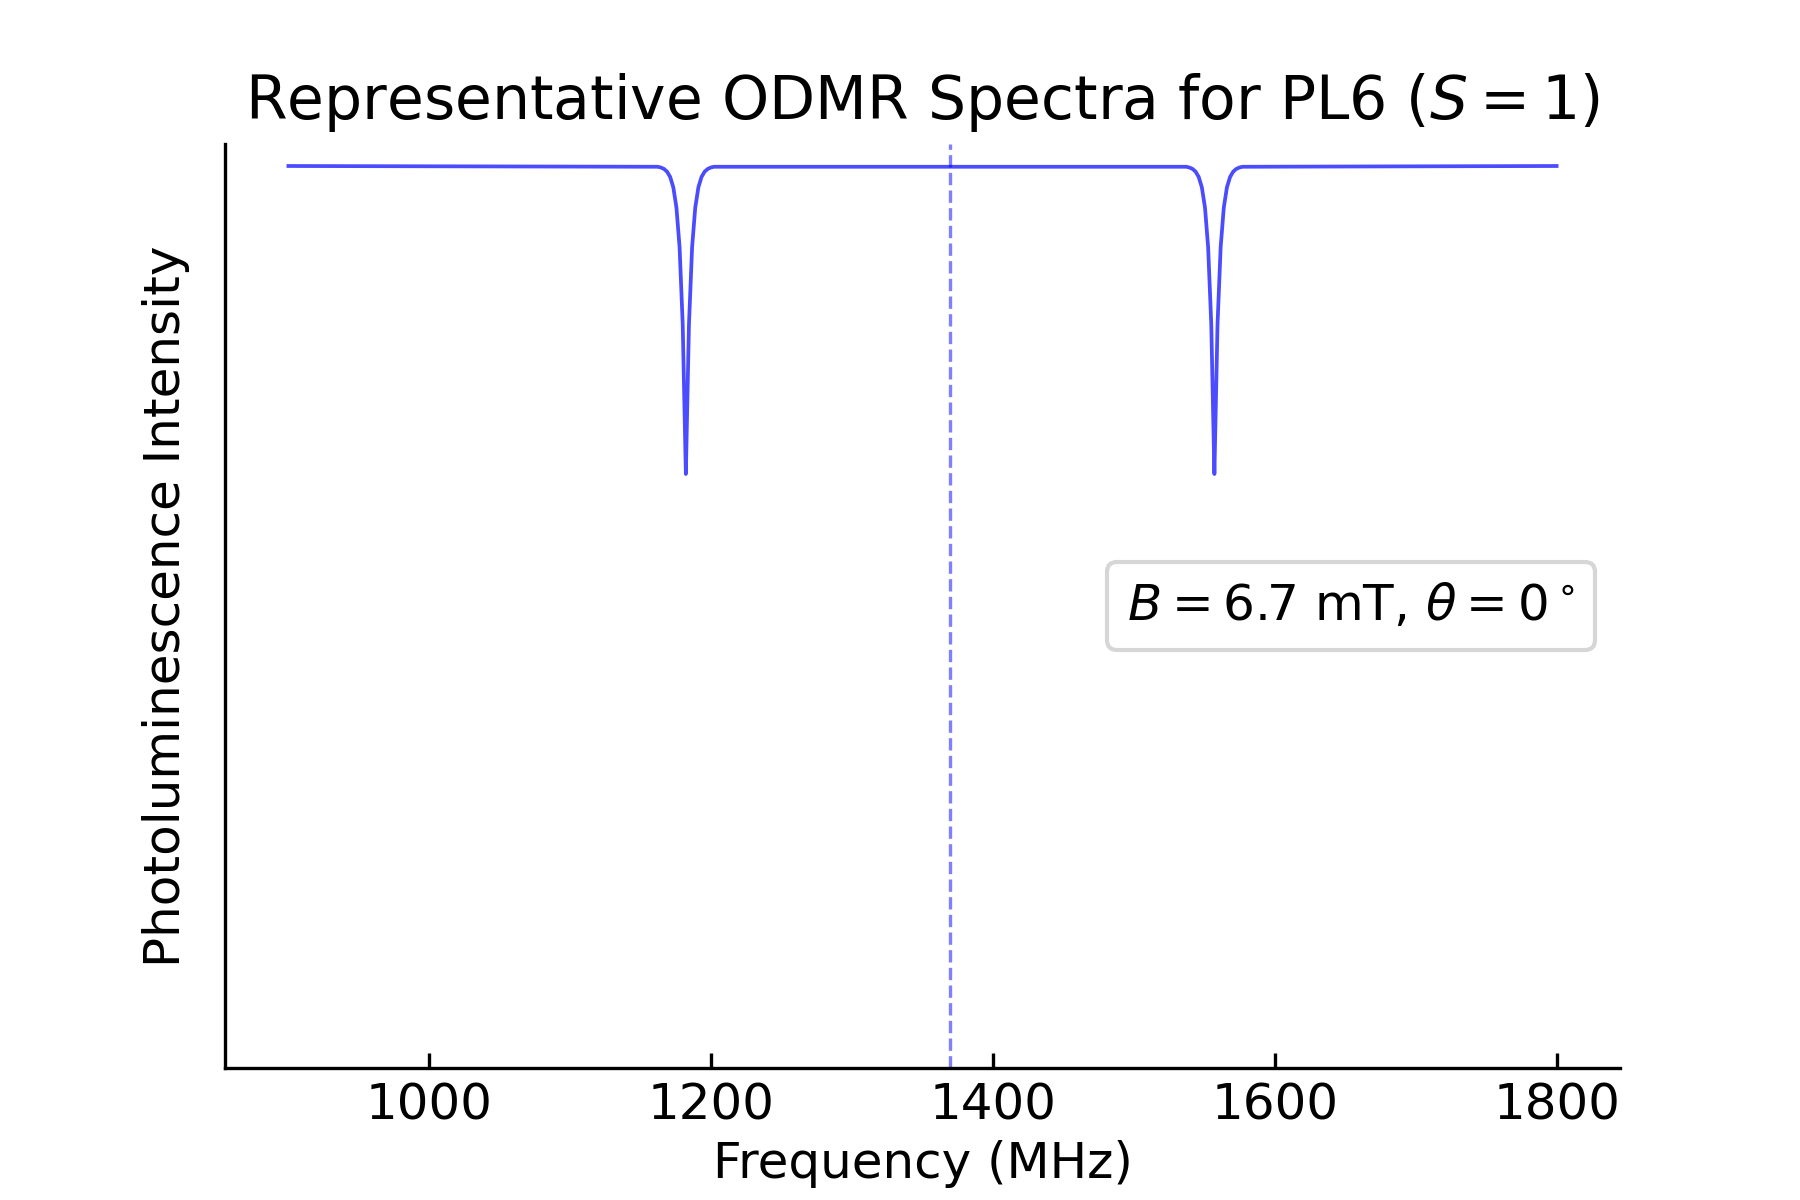
\includegraphics[width=0.49\textwidth]{figures/ODMR-s1magnet-3.png}

    \end{center}
    \caption{Representative PL6 ODMR spectra showing linear dependence of frequency difference on $B\cos\theta$ and the ZFS shifting of the spectra when $\theta > 0$. Dashed vertical line indicates $D$.}\label{fig:linear_zeeman}
\end{figure}
Thus, for CW-ODMR the difference between the two frequencies $f_1 > f_2$ is directly proportional to $B$
\begin{equation}
	f_1 = D + \gamma B,  \quad f_2 = D - \gamma B
	\label{eq:}
\end{equation}

It is then straightforward to calculate $B$ using
\begin{equation}
	B = \frac{f_1 - f_2}{2 \gamma}.
	\label{eq:s1_parallel_magnetometry}
\end{equation}


\subsection{Vector Magnetometry}
By returning to \eqref{eq:s1_magnetometry_hamil_spherical_matrix} it immediately follows from the characteristic equation that eigenvalues $\lambda$ satisfy
\begin{equation}
	0 = \lambda^3 - 2\lambda^2 D + \frac{D (g\mu_b B)^2}{2} + \lambda(D^2 - E^2 - (g\mu_b B)^2) - \frac{1}{2}(g\mu_b B)^2\underbrace{\left(D \cos(2\theta) - 2  E \cos(2\varphi)  \sin^2(\theta)\right)}_{\eta}
	\label{eq:nv_spherical_characteristic_equation}
\end{equation}
where $\eta$ depends only on the ZFS parameters and the vector of the applied $\vec{B}$ field.

This allows a more general determination of $B$ from the ODMR spectra using
\begin{equation}
	B = \frac{\sqrt{\frac{1}{3} \left(f_1^2 - f_1 f_2 + f_2^2 -D^2 -3E^2\right)}}{g \mu_B}.
	\label{eq:spin1_magnet_magnitude}
\end{equation}

Further we may find $\eta$ using
\begin{equation}
	\eta = \frac{-7 D^3 - 4f_1^3 + 6 f_1^2 f_2 + 6f_1 f_2^2 - 4f_2^3 + 3D(9E^2 + f_1^2 -f_1 f_2 + f_2^2)}{9(D^2 + 3E^2 - f_1^2 + f_1f_2 - f_2^2)}.
	\label{eq:}
\end{equation}
Again, exploiting the uniaxial symmetry of our systems we may reduce our expression for $\eta$
\begin{equation}
	\eta = D \cos(2\theta) - 2  E \cos(2\varphi) \sin^2(\theta) \simeq D \cos2\theta
	\label{eq:}
\end{equation}
therefore with just two frequencies and knowledge of the ZFS parameters, whilst a complete vector cannot be reconstructed, we may determine the magnitude and azimuthal angle of an applied $\vec{B}$ field
\begin{equation}
	\theta = \frac{\cos^{-1} (\eta/D)}{2}
	\label{eq:spin1_magnet_theta}
\end{equation}


\begin{summary}{$S=1$ Magnetometry Summary}{sum:spin1magnet}

	We may achieve angle resolved magnetometry using a $S=1$ system provided:
	\begin{enumerate}
        \item We can resolve \textbf{two frequencies} corresponding to the defect in the CW-ODMR spectra.
		\item We know the ZFS parameters $D$ and $E$.

		\item We can determine the magnitude using
		      \begin{equation}
			      \tcbhighmath{B = \frac{\sqrt{\frac{1}{3} \left(f_1^2 - f_1 f_2 + f_2^2 -D^2 -3E^2\right)}}{g \mu_B}.}
			      \tag{\ref{eq:spin1_magnet_magnitude}}
			      % \tcbhighmath{g\mu_b B = \frac{f_1 - f_2}{2 \gamma}}
			      % \tag{\ref{eq:s1_parallel_magnetometry}}
		      \end{equation}
		\item We can determine the azimuthal angle using
		      \begin{equation}
			      \tcbhighmath{
				      \theta = \frac{\cos^{-1} (\eta/D)}{2}.
			      }
			      \tag{\ref{eq:spin1_magnet_theta}}
		      \end{equation}
	\end{enumerate}


\end{summary}
